\chapter{Technical Details and Implementation}
\label{chapter5_technical_details}
\thispagestyle{empty}

\vspace{0.5cm}

In this chapter we show the implementation details of the architecture
used to perform experiments. We try to provide a complete description of the 
parametrization of the components and of the training procedure to ensure 
reproducibility of the experimental results.

\section{Atari Environments}\label{s:atari_envs}
The \textit{Arcade Learning Environment} (ALE) \cite{bellemare2013arcade} is an 
evaluation platform for RL agents.
ALE offers a programmatic interface to hundreds of game environments for the 
\textit{Atari 2600}, a popular home video game console developed in 1977 with 
more than 500 games available, and is simply referred to as 
\textit{Atari environments} (or \textit{games}). 
We use the implementation of ALE provided by the \textit{Gym 0.9.2} package for 
Python 2.7, developed by OpenAI and maintained as an open source project. 
This implementation provides access to the game state in the form of 
$3 \times 110 \times 84$ RGB frames, produced at an internal frame-rate of $60$ 
frames per second (FPS).
When an action is executed in the environment, the simulator repeats the action 
for four consecutive frames of the game and then provides another observation, 
effectively lowering the frame rate from $60$ FPS to $15$ FPS and making the 
effects of actions more evident (Figure \ref{f:sampling}). 
%
\begin{figure}

\includegraphics[width=\textwidth]{pictures/sampling}
\centering
\caption[Sampling frames at a frequency of $\frac{1}{4}$ in \textit{Breakout}]{Sampling frames at a frequency of $\frac{1}{4}$ in \textit{Breakout}.}
\label{f:sampling}
\end{figure}
%
We perform a preprocessing operation on the states similar to that performed
by Mnih et al.\ in DQN \cite{mnih2015human}, in order to include all necessary 
information about the environment and its nominal dynamics in the new state 
representation.
First we convert each RGB observation to a single-channel grayscale 
representation in the discrete 8-bit interval $[0, 255]$ using the 
\textit{ITU-R 601-2 luma transform}:
%
\begin{IEEEeqnarray}{rCl}
    %
    L = \frac{299}{1000}R + \frac{587}{1000}G + \frac{114}{1000}B
    %
\end{IEEEeqnarray}
%
where $R$, $G$, $B$ are the 8-bit \textit{red, green} and \textit{blue} channels
of the image. We then normalize these values in the $[0, 1]$ interval via 
\textit{max-scaling} (i.e.\ dividing each pixel by $255$).
Moreover, we define a rounding threshold $v_{round}$ specific to each game
and we round all pixel values above or below the threshold to $1$ or 
$0$ respectively, reducing the images to a 1-bit color space in order to 
facilitate the training of the AE. 
We also reduce the height of the image by two pixels in order to prevent 
information loss due to a rounding operation performed by the convolution
method used in the AE.
Finally, we concatenate the preprocessed observation to the last three 
preprocessed frames observed from the environment, effectively blowing up the
state space to a $4 \times 108 \times 84$ vector space (Figure \ref{f:state}). 
The initial state for an episode is artificially set as a repetition of the 
first observation provided by the simulator. 
%
\begin{figure}
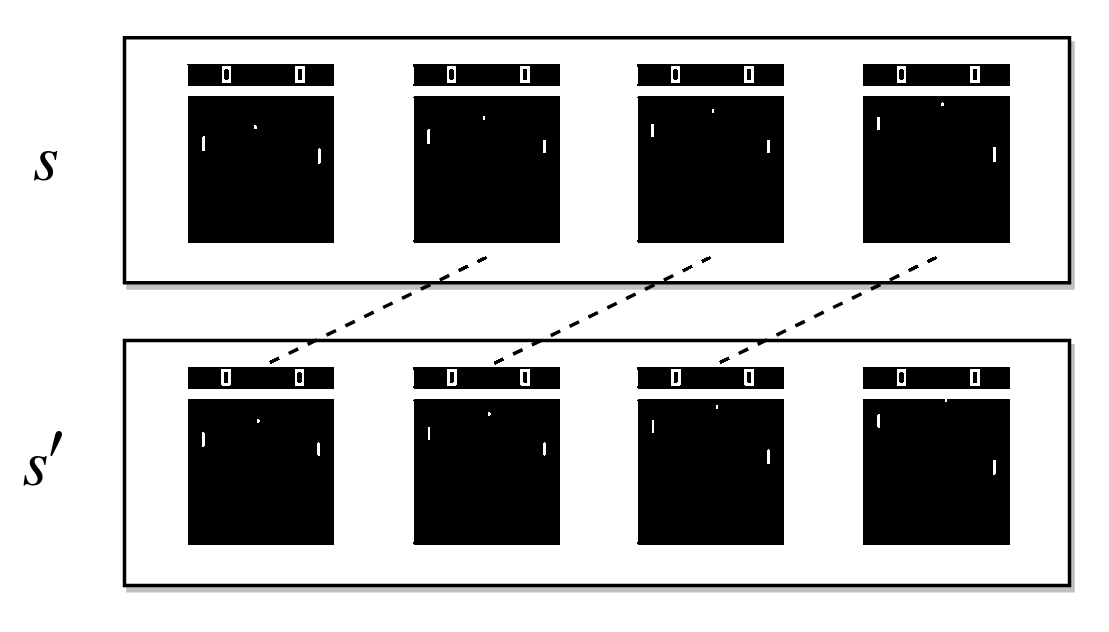
\includegraphics[width=\textwidth]{pictures/state}
\centering
\caption[Two consecutive states in \textit{Pong}]{Two consecutive states 
	$s, s'$ in \textit{Pong}, after the preprocessing operation. Each 
	binary image in a sequence of four is an observation of $108 \times 84$
	pixels, and the full $4 \times 108 \times 84$ tensor is given as input
	and target to the AE. Notice that between the two consecutive states 
	there are three frames in common, with the newest observation appended
	as last frame in $s'$ and the oldest being pushed out.}
\label{f:state}
\end{figure}
%
    
Moreover, in order to facilitate comparisons and improve stability, we remain 
loyal to the methodology used for DQN and perform the same clipping of the 
reward signal in a $[-1, 1]$ interval. 

We also add a tweak to the Gym implementation of ALE in order to fix a 
requirement of some environments of performing some specific actions in 
order to start an episode (e.g.\ in \textit{Breakout} it is required that the 
agent takes action 1 to start the game). We automatically start each episode by 
randomly selecting one of the initial actions of the game and forcing the agent 
to take that action at the beginning of the episode. 

Finally, for those games in which the agent has a lives count, we monitor the 
number of remaining lives provided by the simulator in the \textit{ale.lives}
parameter. For those $(s, a, r, s')$ transitions in which the agent loses a life, 
we consider $s'$ as a terminal state, so that the FQI update will only 
use the reward rather than the full value. 

\section{Autoencoder}\label{s:ae_training_details}
%
\begin{table}
    \centering
    \begin{tabular}{l c c c c c c} 
	\hline
	Type & Input & Output & \# Filters & Filter & Stride & Activation \\ 
	\hline 
	Conv. & $4 \times 108 \times 84$ & $32 \times 26 \times 20$ & $32$ & $8 \times 8$ & $4 \times 4$ & ReLU \\ 
	Conv. & $32 \times 26 \times 20$ & $64 \times 12 \times 9$ & $64$ & $4 \times 4$ & $2 \times 2$ & ReLU \\ 
	Conv. & $64 \times 12 \times 9$ & $64 \times 10 \times 7$ & $64$ & $3 \times 3$ & $1 \times 1$ & ReLU \\ 
	Conv. & $64 \times 10 \times 7$ & $16 \times 8 \times 5$ & $16$ & $3 \times 3$ & $1 \times 1$ & ReLU \\ 
	Flatten	& $16 \times 8 \times 5$ & $640$ & - & - & - & - \\ 
	\hline
	Reshape & $640$ & $16 \times 8 \times 5$ & - & - & - & - \\
	Deconv. & $16 \times 8 \times 5$ & $16 \times 10 \times 7$ & $16$ & $3 \times 3$ & $1 \times 1$ & ReLU \\ 
	Deconv. & $16 \times 10 \times 7$ & $64 \times 12 \times 9$ & $64$ & $3 \times 3$ & $1 \times 1$ & ReLU \\
	Deconv. & $64 \times 12 \times 9$ & $64 \times 26 \times 20$ & $64$ & $4 \times 4$ & $2 \times 2$ & ReLU \\
	Deconv. & $64 \times 26 \times 20$ & $32 \times 108 \times 84$ & $32$ & $8 \times 8$ & $4 \times 4$ & ReLU \\
	Deconv. & $32 \times 108 \times 84$ & $4 \times 108 \times 84$ & $4$ & $1 \times 1$ & $1 \times 1$ & Sigmoid \\
	\hline
    \end{tabular}
    \caption{Layers of the autoencoder with key parameters.}
    \label{t:AE_structure}
\end{table}
%
We use the autoencoder to extract a high level representation $\tilde{S}$ of the
state space in an unsupervised fashion.
We structure the AE to take as input the preprocessed observations from the
environment and predict values on the same vector space.
The first four convolutional layers make up the encoder and perform a 2D 
convolution with the \textit{valid} padding algorithm such that the input of 
each layer (in the format $channels \times height \times width$) is reduced 
automatically across the last two dimensions (height and width) according to the
following formula: 
%
\begin{IEEEeqnarray}{rCl}
    %
    output_i = \lfloor(input_i - filter_i  + stride_i) / stride_i\rfloor
    %
\end{IEEEeqnarray}
%
Since the main purpose of pooling layers is to provide translation invariance to 
the representation of the CNN (meaning that slightly shifted or tilted inputs
are considered the same by the network), here we choose to not use pooling 
layers in order to preserve the precious information regarding the position of
different elements in the game; this same approach was adopted in DQN.
A final \textit{Flatten} layer is added at the end of the encoder to provide a 
1D representation of the feature space, which is reversed before the beginning 
of the decoder. 
The decoder consists of deconvolutional layers with symmetrical filter sizes, 
filter numbers and strides with respect to the encoder. Here the \textit{valid} 
padding algorithm is inversed to expand the representation with this formula:
%
\begin{IEEEeqnarray}{rCl}
    %
    output_i = \lfloor (input_i \cdot stride_i) + filter_i  - stride_i\rfloor
    %
\end{IEEEeqnarray}
% 
A deconvolutional layer is added at the end to reduce the number of channels 
back to the original four, without changing the width and height of the frames 
(i.e.\ using unitary filters and strides). 
All layers in the AE use the \textit{Rectified Linear Unit} (ReLU) 
\cite{nair2010rectified, krizhevsky2012imagenet} nonlinearity as activation 
function, except for the last layer that uses \textit{sigmoids} to limit the 
activations values in the same $[0, 1]$ interval of the input (Figure 
\ref{f:relu_sigmoid}).
Details of the AE layers are summarized in Table \ref{t:AE_structure}.
%
\begin{figure}
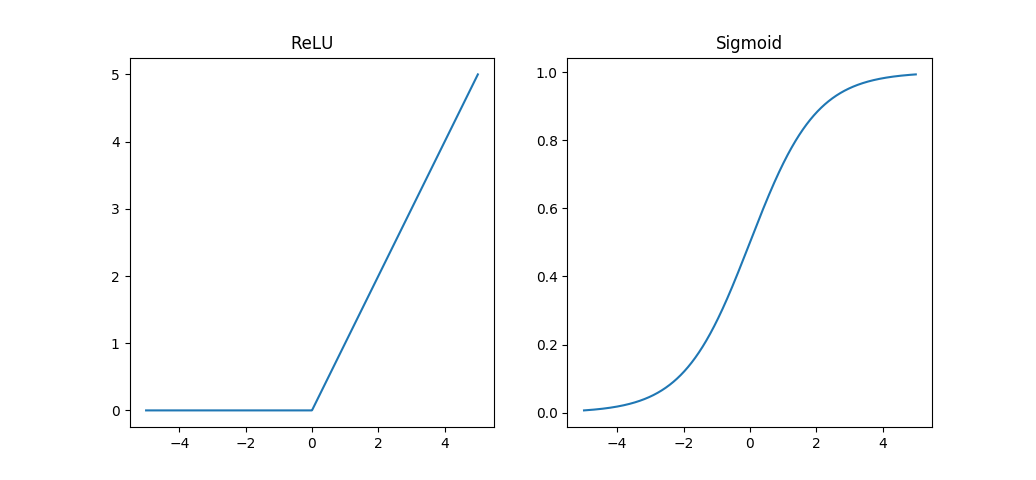
\includegraphics[width=\textwidth]{pictures/relu_sigmoid}
\centering
\caption[The ReLU and Sigmoid activation functions for the AE]{The ReLU and Sigmoid activation functions for the AE.}
\label{f:relu_sigmoid}
\end{figure}
%

We train the AE with the Adam optimization algorithm \cite{kingma2014adam} 
(see Table \ref{t:adam_params} for details on the hyperparameters) set to 
minimize the \textit{binary cross entropy} loss defined as:
%
\begin{IEEEeqnarray}{rCl}
    %
    L(y, \hat y) = - \frac{1}{N} \sum\limits_{n=1}^{N}[y_n log(\hat y_n) + (1-y_n) log(1-\hat y_n)]
    %
\end{IEEEeqnarray}
%
where $y$ and $\hat y$ are vectors of $N$ target and predicted observations in 
the state space. The dataset used for training is a subset of the dataset 
collected for the whole learning procedure described in Algorithm 
\ref{alg:FQI-DSDF}, namely the first elements of the four-tuples $(s, a, r, s') 
\in \mathcal{TS}$ (which are used as input and targets).
%
\begin{table}
    \centering
    \begin{tabular}{l c} 
	\hline
	Parameter & Value \\ 
	\hline 
	Learning rate &  $0.001$ \\
	Batch size & $32$ \\
	Exponential decay rate ($\beta_1$) & $0.9$ \\
	Exponential decay rate ($\beta_2$) & $0.999$ \\
	Fuzz factor ($\varepsilon$) & $10^{-8}$ \\
	\hline
    \end{tabular}
    \caption{Optimization hyperparameters for Adam.}
    \label{t:adam_params}
\end{table}
%
We prevent \textit{overfitting} of the training set by monitoring the 
performance of the AE on a held-out set of validation samples that amounts to
roughly $10\%$ of the training data, and stopping the procedure when the 
validation loss does not improve by at least $10^{-5}$ for five consecutive 
training epochs. 

\section{Tree-based Recursive Feature Selection}
% I/O (?)
% Parametrization of trees
% Significance
We use the RFS algorithm to reduce the state space representation computed by 
the AE down to the feature space $\hat{S}$.
We base both the feature ranking method $FR$ and the model $\hat{f}$, used for
computing the descriptiveness of the features, on the supervised Extra-Trees 
algorithm (cf.\ Section \ref{s:extra-trees}).

The feature ranking approach with Extra-Trees is based on the idea of scoring
each input feature by estimating the variance reduction produced anytime that 
the feature is selected during the tree building process. The ranking score is
computed as the percentage of variance reduction achieved by each feature over 
the $M$ trees built by the algorithm.

At the same time, Extra-Trees is a sufficiently powerful and computationally 
efficient supervised learning algorithm to use as $\hat{f}$.
Note that in general $FR$ and $\hat{f}$ could be different algorithms with 
different parametrizations, but Castelletti et al.\ use the same regressor for 
both tasks (as does the code implementation of RFS and IFS that we used for 
experiments), and we therefore complied with this choice.
The parametrization of Extra-Trees for $FR$ and $\hat{f}$ is reported in Tables
\ref{t:RFS_tree_params}\footnote{We use two different values for the minimum 
number of samples required to split an internal node or a leaf.} and 
\ref{t:RFS_extra_params}, respectively for the parameters of the base trees used
to build the ensemble and the Extra-Trees algorithm itself (cf.\ Section 
\ref{s:extra-trees}).
%
\begin{table}	
    \centering
    \begin{tabular}{l c} 
	\hline
	Parameter & Value \\ 
	\hline 
	Scoring method &  Variance reduction \\
	Max tree depth & None \\
	$n_{min}$ (node) & $5$\\
	$n_{min}$ (leaf) & $2$ \\
	\hline
    \end{tabular}
    \caption{Parameters for base estimators in Extra-Trees (RFS).}
    \label{t:RFS_tree_params}
\end{table}
%
%
\begin{table}
    \centering
    \begin{tabular}{l c} 
	\hline
	Parameter & Value \\ 
	\hline 
	$M$ (Number of base estimators) & $50$ \\
	$K$ (Number of randomly selected attributes) &  All available attributes \\
	\hline
    \end{tabular}
    \caption{Parameters for Extra-Trees (RFS).}
    \label{t:RFS_extra_params}
\end{table}
%
We use the $R^2$ metric defined in Equation \eqref{e:R2} to compute the ability
of the selected features to describe the target, in $K$-fold cross validation 
over the training set $\mathcal{D}$. We compute a confidence interval over the 
scores of the validation predictions as:
\begin{IEEEeqnarray}{rCl}
    %
    CI = \sqrt{\frac{1}{|\mathcal{D}|} \sum\limits_{i = 1}^{|\mathcal{D}|} (R^2)^2 \cdot (\frac{1}{|\mathcal{D}|} \sum\limits_{i = 1}^{|\mathcal{D}|} (R^2))^2}
    %
\end{IEEEeqnarray}
and we adapt the stopping condition of RFS by setting $\epsilon = CI + CI_{old}$ 
(where the suffix $old$ has the same meaning as in Algorithm \ref{alg:IFS}) so
that the condition becomes $R^2 - CI < R^2_{old} - CI_{old}$.
We also multiply $\epsilon$ by a \textit{significance} factor $\xi$ in order to
control the amount of variance that a feature must explain in order to be added 
to the selection: higher values of $\xi$ means that the selection will yield a 
smaller subset composed exclusively of very informative features (even if the 
overall amount of variance explained is not necessarily the whole possible 
amount).
The hyperparameters used for RFS are reported in Table \ref{t:RFS}.
%
\begin{table}
    \centering
    \begin{tabular}{l c} 
	\hline
	Parameter & Value \\ 
	\hline 
	$K$ (for $K$-fold cross-validation) & $3$ \\
	$\xi$ (significance) &  0.5 \\
	\hline
    \end{tabular}
    \caption{Parameters for RFS.}
    \label{t:RFS}
\end{table}
%

\section{Tree-based Fitted Q-Iteration}
We use the FQI algorithm to learn an approximation of the $Q$ function from the
compressed and reduced state space extracted by the previous two modules. 
For consistency with the feature selection algorithm, we use the Extra-Trees 
learning method as function approximator for the action-value function.
The model is trained to map the 1D compressed feature space $\hat{S}$ to the 
$|A|$-dimensional action-value space $\mathbb{R}^{|A|}$, and we use the action 
identifiers to select the single output value of our approximated $\hat{Q}$ 
function. 
The parametrization of the decision trees built for the ensemble is reported in
Table \ref{t:FQI_tree_params} and the parametrization specific to Extra-Trees 
is reported in Table \ref{t:FQI_extra_params} (cf.\ Section \ref{s:extra-trees}).
%
\begin{table}	
    \centering
    \begin{tabular}{l c} 
	\hline
	Parameter & Value \\ 
	\hline 
	Scoring method &  Variance reduction \\
	Max tree depth & None \\
	$n_{min}$ (node) & $2$\\
	$n_{min}$ (leaf) & $1$ \\
	\hline
    \end{tabular}
    \caption{Parameters for base estimators in Extra-Trees (FQI).}
    \label{t:FQI_tree_params}
\end{table}
%
%
\begin{table}
    \centering
    \begin{tabular}{l c} 
	\hline
	Parameter & Value \\ 
	\hline 
	$M$ (Number of base estimators) & $100$ \\
	$K$ (Number of randomly selected attributes) &  All available attributes \\
	\hline
    \end{tabular}
    \caption{Parameters for Extra-Trees (FQI).}
    \label{t:FQI_extra_params}
\end{table}
%

Since the FQI procedure introduces a small bias to the action-value estimate at 
each iteration (due to approximation errors), we implement an \textit{early 
stopping} procedure based on the evaluation of the agent's performance.
Every fixed number of iterations we evaluate the performance of an 
$\varepsilon$-greedy policy (with $\varepsilon = 0.05$) based on the current 
partial approximation $\hat{Q}_i$, by composing all the modules in the pipeline 
to obtain the full $Q$ as per Equation \eqref{eq:final_output}. 
If the agent's performance does not improve for five consecutive evaluations, we 
stop the training and produce the best performing estimation as output to the 
training phase.
The performance is evaluated by running the policy for five episodes and 
averaging the clipped cumulative return of each evaluation episode. 

Finally, we consider a discount factor $\gamma = 0.99$ for the MDP in order to 
give importance to rewards in a sufficiently large time frame. 

\section{Evaluation}
An evaluation step is run after each training step of the full procedure.
Similarly to what we do to evaluate the agent's performance during the training
of FQI, here we use an $\varepsilon$-greedy policy with $\varepsilon = 0.05$ 
based on the full $Q$ composition of Equation \eqref{eq:final_output}.
The reason for using a non-zero exploration rate during evaluation is that ALE
provides a fully deterministic initial state for each episode, and by using a 
deterministic policy we would always observe the same trajectories (thus leading
to overfitting to the best policy from the initial state, rather than a generic
good policy from any state). Using a non-zero exploration rate allows us to 
assess the agent's capability of playing effectively in any state of the game, 
and of correcting its behavior after an (albeit artificial) mistake.

We let the agent experience $N$ separate episodes under the $\varepsilon$-greedy 
policy, and for each episode we consider the cumulative clipped return and the
number of steps occurred. The mean and variance of these two metrics across the 
$N$ episodes provide us with insights on the agent's performance: a high average 
return obviously means that the algorithm has produced a good policy, but at the
same time a low variance in the number of steps could indicate that the agent is 
stuck in some trivial policy (e.g. take always the same action) which causes the
episodes to be essentially identical, even accounting for the non-zero 
exploration rate. The latter aspect, while not negative in general, can help in 
the initial steps of experiments to detect potential problems in the 
implementation.

Evaluation parameters are summarized in Table \ref{t:eval}.
%
\begin{table}[h]
    \centering
    \begin{tabular}{l c} 
	\hline
	Parameter & Value \\ 
	\hline 
	Exploration rate $\varepsilon$ & $0.05$ \\
	$N$ &  $10$ \\
	\hline
    \end{tabular}
    \caption{Parameters for evaluation.}
    \label{t:eval}
\end{table}
%
